\documentclass[a4paper,14pt]{article}

\usepackage[T2A]{fontenc}
\usepackage[utf8]{inputenc}
\usepackage[russian]{babel}
\usepackage{graphicx}
\usepackage[left=1cm,right=1cm,bottom=1cm,top=2cm]{geometry}
\usepackage{hyperref}
\title{Приложение к ленте времени по Возрождению}
\author{Егор Федоров, P3115}
\date{Октябрь 2022 г.}

\usepackage{fancyhdr}
\fancyhead[L]{Федоров Егор, P3115}
\fancyhead[R]{Приложение к ленте времени по Возрождению}
\fancyfoot{}

\begin{document}
\pagestyle{fancy}
\section*{Возрождение в России}

\begin{enumerate}
    \item Церковь Спаса Преображения на Ильине улице (см. рис.~\ref{fig:rus:1}), 1374 г.
    \item Церковь Василия на Горке (Псков) (см. рис.~\ref{fig:rus:2}), 1413-1415 гг.
    \item «Троица» (см. рис.~\ref{fig:rus:3}), Андрей Рублей, 1411 г. или 1425-1427 гг.
    \item Успенский собор (Московский кремль) (см. рис.~\ref{fig:rus:4}), Аристотель Фьораванти, 1475-1479 гг.
    \item Благовещенский собор (Московский кремль) (см. рис.~\ref{fig:rus:5}), Кривцов и Мышкин, 1484-1489 гг.
    \item Гранитовая палата (см. рис.~\ref{fig:rus:6}), Марк Фрязин и Пьетро Антонио Солари, 1487-1491 гг.
    \item Архангельский собор (Московский кремль) (см. рис.~\ref{fig:rus:7}), Алевиз Новый, 1505-1508 гг.
    \item Новодевичий монастырь (см. рис.~\ref{fig:rus:8}), 1524 г.
    \item Храм Василия Блаженного (см. рис.~\ref{fig:rus:9}), 1555-1561 гг.
    \item Успенский собор (см. рис.~\ref{fig:rus:10}), 1585 г.
\end{enumerate}

\section*{Итальянское Возрождение}
\begin{enumerate}
\item «Поцелуй Иуды» (см. рис.~\ref{fig:italy:1}), Джотто, 1306 год, находится в Капелле Скровеньи
\item «Распятие» (см. рис.~\ref{fig:italy:2}), Пьетро Лоренцетти, 1320 год, Сан-Франческо Ассизи
\item «Вход Господень в Иерусалим» (см. рис.~\ref{fig:italy:3}), Пьетро Лоренцетти, 1320 год, Сан-Франческо Ассизи
\item «Чудо со статиром» (см. рис.~\ref{fig:italy:4}), Мазаччо, 1425-1427 года
\item «Положение во гроб» (см. рис.~\ref{fig:italy:5}), Фра Беато Анджелико, около 1438-1440 гг.
\item «Мадонна на троне с Младенцем и двумя ангелами» (см. рис.~\ref{fig:italy:6}), Филиппо Липпи, 1440 г.
\item «Мадонна с Младенцем» (см. рис.~\ref{fig:italy:7}), Филиппо Липпи, ок. 1465 г.
\item «Вручение ключей апостолу Петру» (см. рис.~\ref{fig:italy:8}), Пьетро Перуджино, около 1482 года, Сикстинская капелла=
\item «Вознесение Девы Марии» (см. рис.~\ref{fig:italy:9}), Тициан, 1516-1518 года
\item «Вознесение Девы Марии» (см. рис.~\ref{fig:italy:10}), Корреджо, 1530 год
\end{enumerate}
\section*{Северное Возрождение}
\begin{enumerate}
\item «Гентский алтарь» (см. рис.~\ref{fig:north:1}), Хуберт ван Эйк и Ян ван Эйк, 1432 г.
\item «Портрет четы Арнофильнии» (см. рис.~\ref{fig:north:2}), Ян ван Эйк, 1432 г.
\item <<Снятие с креста» (см. рис.~\ref{fig:north:3}), Рогир ван дер Вейден, ок. 1435-1440 гг.
\item «Сад земных наслаждений» (триптих Босха) (см. рис.~\ref{fig:north:4}), Иероним Босх, 1500-1510 гг.
\item «Изенгемский алтарь» (см. рис.~\ref{fig:north:5}), Маттиас Грюневальд, 1512-1515 гг.
\item «Адам и Ева. Грехопадение» (см. рис.~\ref{fig:north:6}), Лукас Кранах Старший, 1527 г. 
\item «Портрет Генриха VIII» (см. рис.~\ref{fig:north:7}), Ганс Гольбейн Младший, 1537 г.
\item «Охотники на снегу» (см. рис.~\ref{fig:north:8}), Питер Брейгель Старший, 1565 г.
\item «Притча о слепых» (см. рис.~\ref{fig:north:9}), Питер Брейгель Старший, 1568 г.
\item «Калеки» (см. рис.~\ref{fig:north:10}), Питер Брейгель Старший, 1568 г.

\end{enumerate}
\begin{figure}[ht]
    \centering
    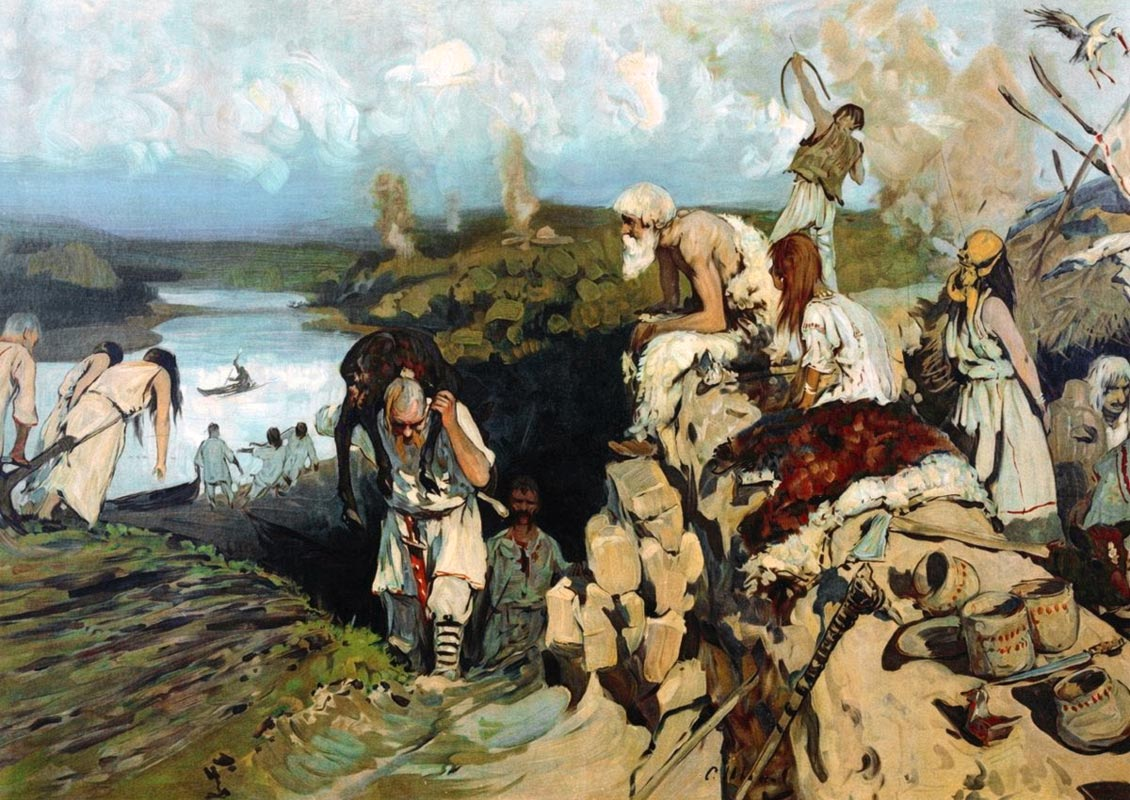
\includegraphics[width=0.45\textwidth]{img/rus/Living_of_East_Slavs_by_Ivanov.jpg}
    \caption{Жилье восточных славян}
    \label{fig:slavs}
\end{figure}

\begin{figure}[ht]
    \centering
    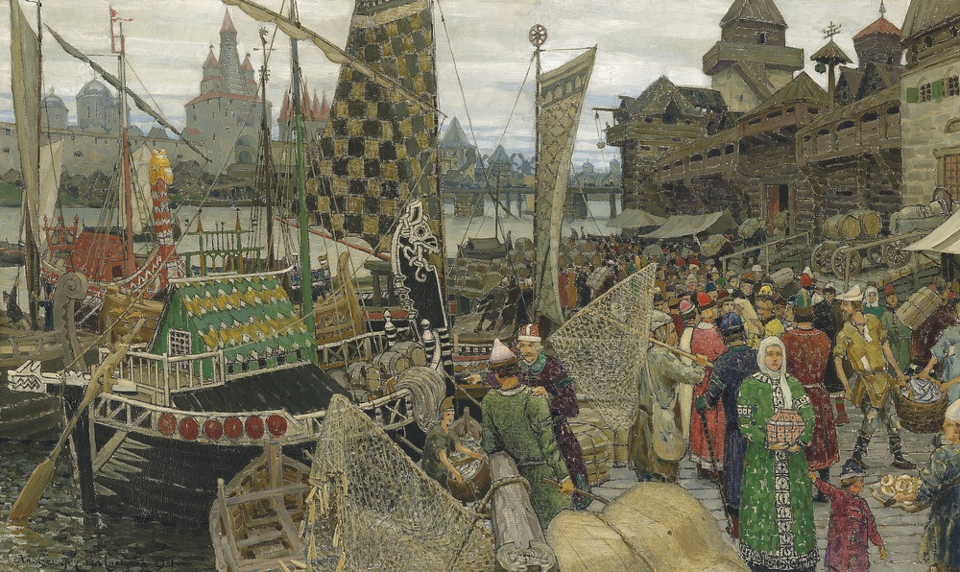
\includegraphics[width=0.45\textwidth]{img/rus/novgorod.png}
    \caption{Великий Новгород}
    \label{fig:novrogod}
\end{figure}

\begin{figure}[ht]
    \centering
    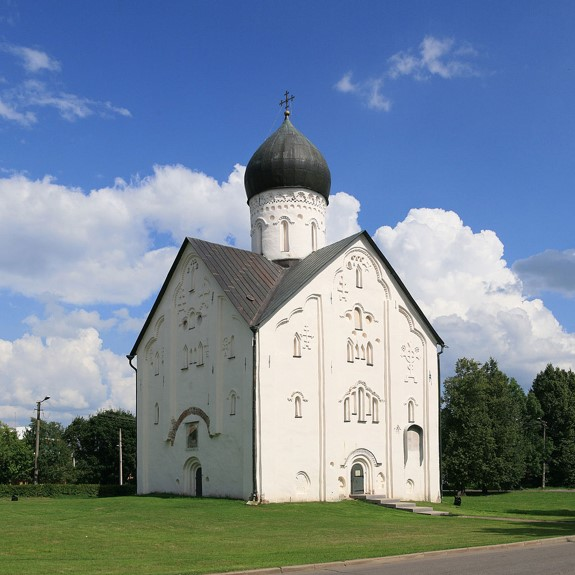
\includegraphics[width=0.45\textwidth]{img/rus/1.jpg}
    \caption{Призвание варягов}
    \label{fig:summon}
\end{figure}

\begin{figure}[ht]
    \centering
    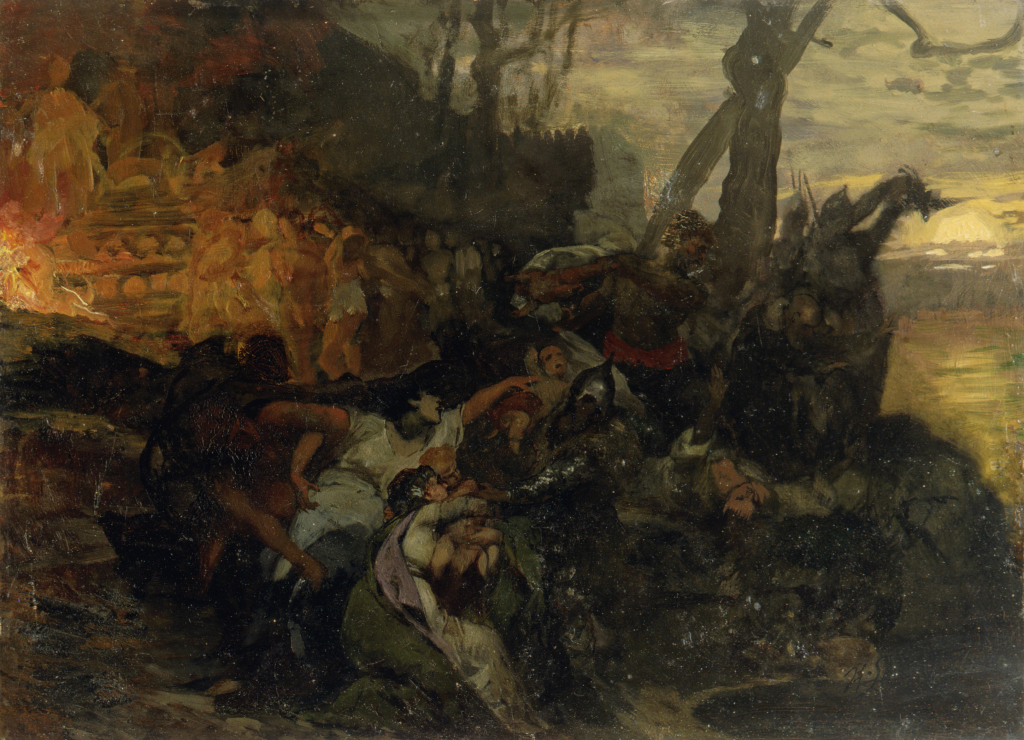
\includegraphics[width=0.45\textwidth]{img/rus/1afa34a7f984eeabdbb0a7d494132ee5_x1.png}
    \caption{Тризна дружинников Святослава после боя под Доростолом в 971 году}
    \label{fig:trizna}
\end{figure}

\begin{figure}[ht]
    \centering
    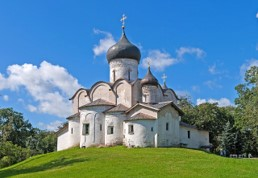
\includegraphics[width=0.45\textwidth]{img/rus/2.jpg}
    \caption{Крещение Руси}
    \label{fig:chresh}
\end{figure}

\begin{figure}[ht]
    \centering
    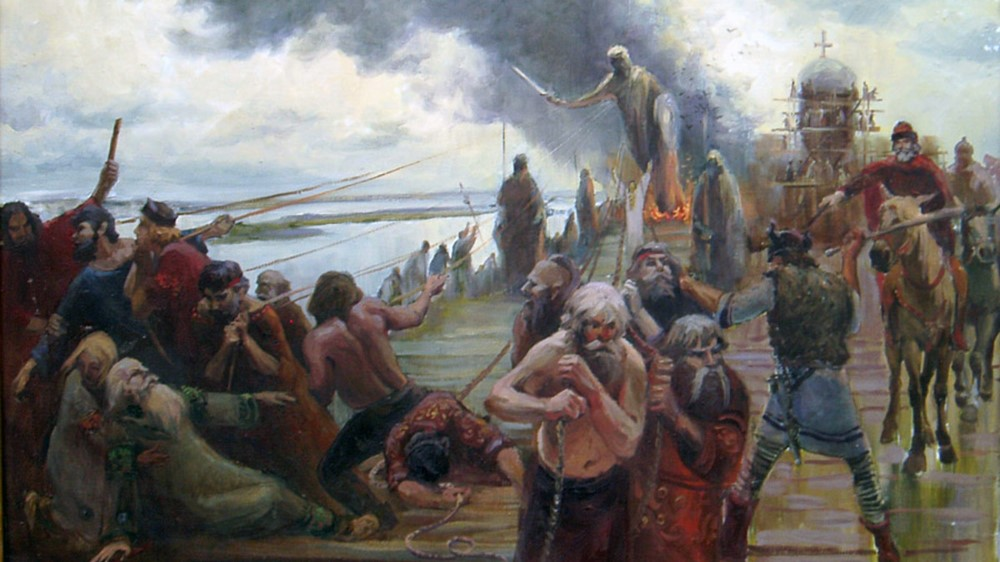
\includegraphics[width=0.45\textwidth]{img/rus/sverzh.jpg}
    \caption{Свержение идолов в Киеве}
    \label{fig:sverzh}
\end{figure}

\begin{figure}[ht]
    \centering
    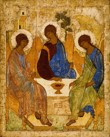
\includegraphics[width=0.45\textwidth]{img/rus/3.jpg}
    \caption{Битва на реке Немиге}
    \label{fig:nemiga}
\end{figure}

\begin{figure}[ht]
    \centering
    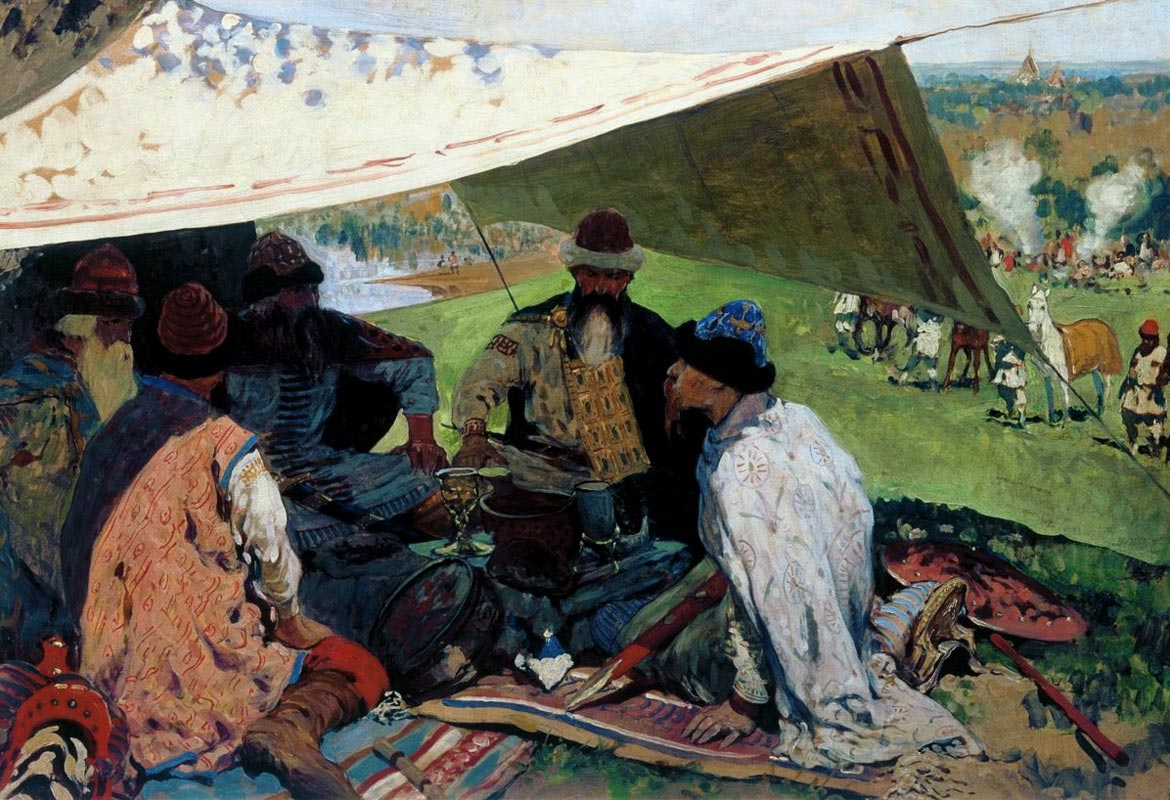
\includegraphics[width=0.45\textwidth]{img/rus/uvetichi.jpg}
    \caption{Русские князья заключают мир в Уветичах}
    \label{fig:uvetichi}
\end{figure}

\begin{figure}[ht]
    \centering
    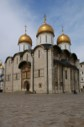
\includegraphics[width=0.45\textwidth]{img/rus/4.jpg}
    \caption{Битва при Салнице}
    \label{fig:salnitsa}
\end{figure}

\begin{figure}[ht]
    \centering
    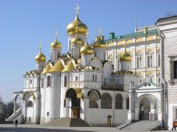
\includegraphics[width=0.45\textwidth]{img/rus/5.jpg}
    \caption{Битва при Калке}
    \label{fig:kalka}
\end{figure}


\clearpage


\begin{figure}[ht]
    \centering
    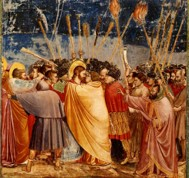
\includegraphics{img/italiy/1.jpg}
    \caption{Поцелуй Иуды}\label{fig:italy:1}
\end{figure}

\begin{figure}[ht]
    \centering
    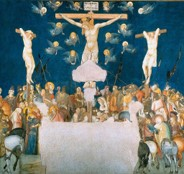
\includegraphics{img/italiy/2.jpg}
    \caption{Распятие}\label{fig:italy:2}
\end{figure}

\begin{figure}[ht]
    \centering
    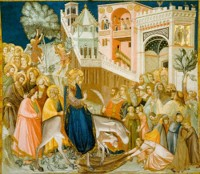
\includegraphics{img/italiy/3.jpg}
    \caption{Вход Господень в Иерусалим}\label{fig:italy:3}
\end{figure}

\begin{figure}[ht]
    \centering
    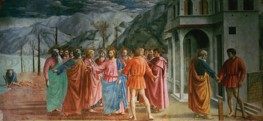
\includegraphics{img/italiy/4.jpg}
    \caption{Чудо со статиром}\label{fig:italy:4}
\end{figure}

\begin{figure}[ht]
    \centering
    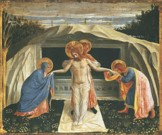
\includegraphics{img/italiy/5.jpg}
    \caption{Положение во гроб}\label{fig:italy:5}
\end{figure}

\begin{figure}[ht]
    \centering
    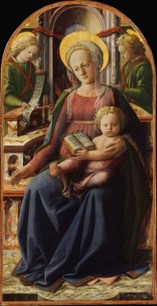
\includegraphics{img/italiy/6.jpg}
    \caption{Мадонна на троне с Младенцем и двумя ангелами}\label{fig:italy:6}
\end{figure}

\begin{figure}[ht]
    \centering
    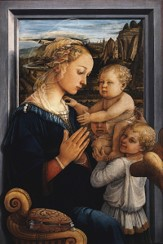
\includegraphics{img/italiy/7.jpg}
    \caption{Мадонна с Младенцем}\label{fig:italy:7}
\end{figure}

\begin{figure}[ht]
    \centering
    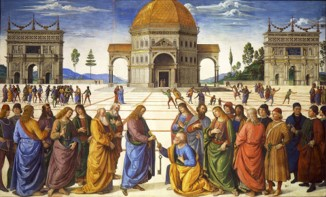
\includegraphics{img/italiy/8.jpg}
    \caption{Вручение ключей апостолу Петру}\label{fig:italy:8}
\end{figure}

\begin{figure}[ht]
    \centering
    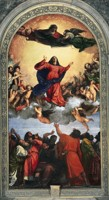
\includegraphics{img/italiy/9.jpg}
    \caption{Вознесение Девы Марии}\label{fig:italy:9}
\end{figure}

\begin{figure}[ht]
    \centering
    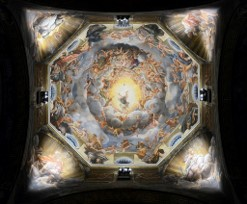
\includegraphics{img/italiy/10.jpg}
    \caption{Вознесение Девы Марии}\label{fig:italy:10}
\end{figure}
\clearpage

\begin{figure}[ht]
    \centering
    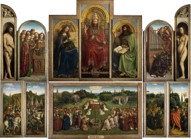
\includegraphics{img/northern/1.jpg}
    \caption{Гентский алтарь}
    \label{fig:north:1}
\end{figure}

\begin{figure}[ht]
    \centering
    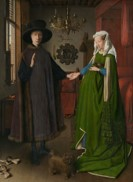
\includegraphics{img/northern/2.jpg}
    \caption{Портрет четы Арнофильнии}
    \label{fig:north:2}
\end{figure}

\begin{figure}[ht]
    \centering
    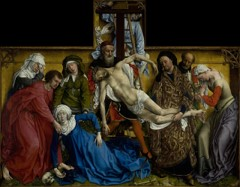
\includegraphics{img/northern/3.jpg}
    \caption{Снятие с креста}
    \label{fig:north:3}
\end{figure}

\begin{figure}[ht]
    \centering
    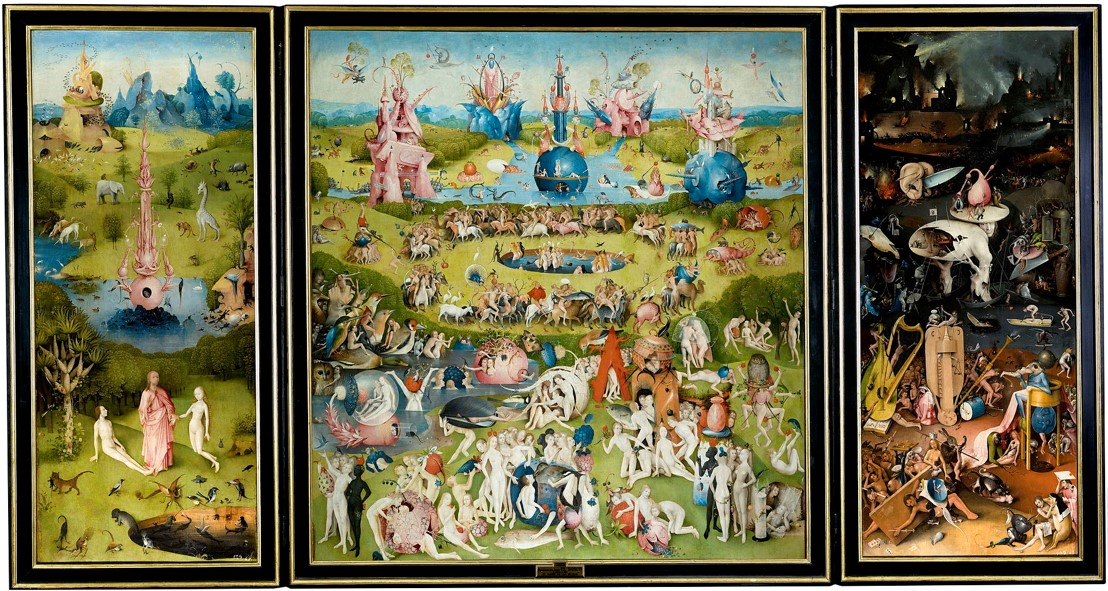
\includegraphics{img/northern/4.jpg}
    \caption{Сад земных наслаждений}
    \label{fig:north:4}
\end{figure}

\begin{figure}[ht]
    \centering
    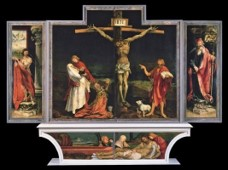
\includegraphics{img/northern/5.jpg}
    \caption{Изенгемский алтарь}
    \label{fig:north:5}
\end{figure}

\begin{figure}[ht]
    \centering
    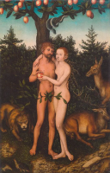
\includegraphics{img/northern/6.png}
    \caption{Адам и Ева. Грехопадение}
    \label{fig:north:6}
\end{figure}

\begin{figure}[ht]
    \centering
    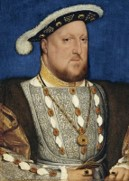
\includegraphics{img/northern/7.jpg}
    \caption{Портрет Генриха VIII}
    \label{fig:north:7}
\end{figure}

\begin{figure}[ht]
    \centering
    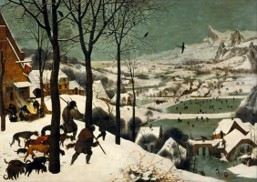
\includegraphics{img/northern/8.jpg}
    \caption{Охотники на снегу}
    \label{fig:north:8}
\end{figure}

\begin{figure}[ht]
    \centering
    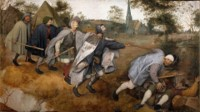
\includegraphics{img/northern/9.jpg}
    \caption{Притча о слепых}
    \label{fig:north:9}
\end{figure}

\begin{figure}[ht]
    \centering
    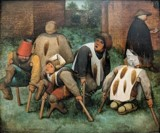
\includegraphics{img/northern/10.jpg}
    \caption{Калеки}
    \label{fig:north:10}
\end{figure}

\end{document}